\section{이론적 배경}
%\section{Theoretical Background}

\subsection{조파 수조와 조파기}
조파 수조는 조파기가 달린 모형 실험용 수조로 해안 혹은 연안에서의 여러 현상을 축소하여 재현 및 실험하기 위한 장치이다. 정밀한 실험을 위해서 기업체나 연구실에서는 큰 스케일로 제작하기도 한다. 주로 선박의 안정성이나 연안에 설치한 구조물의 내구성 등을 시험할 때 맞는 환경을 조성해준다. 초기에는 실험적으로 만들어졌으나 유체 관련 연구가 진행되면서 이론적인 분석이 추가되었다. 
%본교에서 제작한 조파 수조는 파의 진행방향이 한 방향이며 2차원 조파 수조라고 부른다. 

소규모로 운영이 용이하며 비교적 정확한 파를 생성하고 변화를 관찰하기 위해서는 파의 진행방향이 한 방향인 2차원 조파 수조가 적합하다. 2차원 조파 수조를 이용하여 파 특성에 관한 기본 연구나 파와 물체 간의 상호작용에 대한 실험 연구를 충분히 수행할 수 있다. 

\begin{figure}[htbp]
\begin{center}
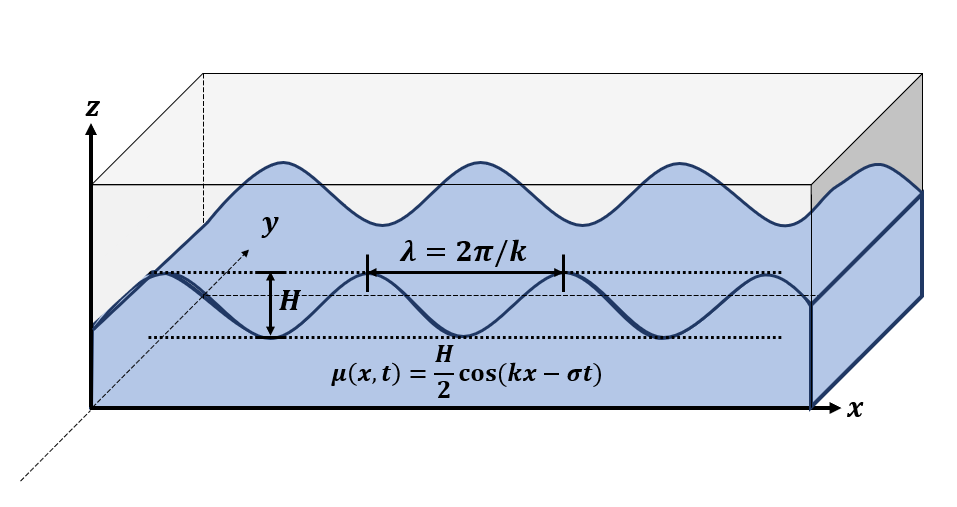
\includegraphics[width=10cm, trim={0 1.8cm 0 1.5cm}, clip]{Water_Tank(Illustrated).png}
\end{center}
\caption{조파 수조 모식도}
\label{Fig01}
\end{figure}
%해파를 만들때 현상을 재현하기 위한 환경을 조성하며 
조파기는 조파 수조에서 파를 생성하는 장치이다. 조파기는 판의 운동 방식에 따라 플랩형, 피스톤형, 플런저형 등이 있다. 피스톤형 조파기는 연안 환경에서의 실험에 자주 사용되는 천해파를 생성하기 용이하다. 피스톤형 조파기에서 파를 생성하는 조파판의 모든 요소는 일관적으로 수평 운동을 한다. 또, 판의 수평 운동 범위를 스트로크라고 하며 $S_0$로 쓰도록 한다 (단, 이는 판의 각 부분이 모두 함께 운동하는 경우에 해당한다).

% 세 종류의 조파기를 보여주는 그림이 필요함.

\subsection{조파 이론(wave maker theory)}

조파 이론은 여러 종류의 조파기가 발생하는 파도의 특성과 개형을 알아보는 것을 목표로 한다\cite{dean1991water} \cite{zhang2007deterministic} \cite{ojk2018}.
2차원 조파 수조에서 피스톤형 조파기가 발생시키는 파도는 여러 방정식을 통해 구할 수 있다. 제일 보편적인 방식은 속도 퍼텐셜 $\phi(x, y, z, t)$를 정의하고 이에 대한 라플라스 방정식과 여러 경계조건을 적용하는 것이다. 방정식을 풀면 속도 퍼텐셜은 다음과 같이 정해진다.

\begin{equation} \label{eq:1}
{
\phi(x, z, t) = A\cosh{[k(h+z)]}\sin(kx-\sigma t) +
\cos(\sigma t){\sum_{n=1}^{\infty}} C_n e^{-k_3 x} \cos{[k_3 (z+h)]} 
}
\end{equation}

%$$\phi(x, z, t) = A\cosh{[k(h+z)]}\sin(kx-\sigma t) + $$
%$$\cos(\sigma t){\sum_{n=1}^{\infty}} C_n e^{-k_3 x} \cos{[k_3 (z+h)]}  $$

파동은 $x$방향으로 진행하며 $h$는 수심이고 $k$는 파수, $\sigma$는 각진동수이다. 그외의 문자는 상수이며 식(\ref{eq:1})로부터 발생파의 변위 식을 다음과 같이 쓸 수 있다.

\begin{equation} \label{eq:2}
{
\mu(x, t) = {{1 \over g}{{\partial \phi} \over {\partial t}}|_{z=0} } = \frac{A \sigma}{g} \cosh(kh) \cos(kx-\sigma t) +
\sin(\sigma t) {\sum_{n=1}^{\infty}} \frac{\sigma C_n}{g} e^{-k_3 x} \cos(k_3 h)
}
\end{equation}

%$$\mu(x, t) = \frac{A \sigma}{g} \cosh(kh) \cos(kx-\sigma t) + $$
%$$\sin(\sigma t) {\sum_{n=1}^{\infty}} \frac{\sigma C_n}{g} e^{-k_3 x} cos(k_3 h) $$

식 (\ref{eq:1}), (\ref{eq:2}) 모두 첫 항은 진행파, 두 번째 항은 정상파를 의미한다. 정상파의 $k_3$은 진팽파의 분산관계식을 정상파 파수로 변환한 식에서 구할 수 있으며 $\sigma ^2 = -g k_3 \tan{k_3 h}$의 해이다. 하지만 제일 큰 해에 대해서 감쇠되는 비율 $\exp{(-k_{3}x)}$가 $x=2h$일 때 $0.04$, $x=3h$일 때 0.009 수준으로 급감하며 본 연구에서는 수조 길이가 6$m$, 수심이 약 15$cm$ 수준이므로 정상파는 무시할 수 있다. 또, 미분방정식의 각각의 고유함수에 대해 일차 근사를 적용하여 파고 $H$를 다음과 같이 표현할 수 있다.

\begin{equation} \label{eq:4}
H = \frac{4 S_0 \sin h{kh}}{\sin h{2kh}+2kh} \left(\sin h{k[z_d - h]} - \sin h{k[z_u - h]}\right)
\end{equation}

%$$H = \frac{4 S_0 \sin h{kh}}{\sin h{2kh}+2kh} (\sin h{k[z_d - h]} - \sin h{k[z_u - h]}) $$

$z_d$는 조파판 하단의 깊이, $z_u$는 조파판 상단의 깊이이며 본 연구의 경우 조파판이 수심 전체에 걸쳐 존재하므로 $z_d = h$, $z_u = 0$이고 파고와 파동 함수는 다음과 같다.

\begin{equation} \label{eq:5}
{
    \frac{H}{S_0}=\frac{4 \sinh^2 k h}{\sinh 2kh + 2kh}
     = \frac{4 \sinh^2 z}{\sinh 2z+2 z}, ~z=kh
}
\end{equation}

\begin{equation} \label{eq:6}
{
    \mu(x, t)=\frac{H}{2} \cos (k x-\sigma t)
}
\end{equation}

%$$\frac{H}{S_0}=\frac{4 \sinh ^2 k h}{\sinh k h+2 k h}, \mu(x, t)=\frac{H}{2} \cos (k x-\sigma t)$$

$S_0,~h$는 구조적인 값이며 조절이 가능하다. 또, 파수 $k$와 각진동수 $\sigma$는 분산 관계식을 만족하므로 결론적으로는 $\sigma$와 $S_0$, $h$를 정하면 된다. 조파판 또한 sin형으로 움직이도록 경계조건으로 반영되었으며 이 경우 판의 진동 변위는 다음과 같다.

\begin{equation} \label{eq:7}
{
    x = {{S_0}\over2} \sin{\sigma t}
}
\end{equation}

하지만 이는 심해파의 경우이다. 여러 경계조건과 근사를 하기 위한 조건이며 심해파는 간단하게 $h/\lambda > 1/2$인 파를 의미하기도 한다. 이와 반대로 천해파는 $h/\lambda < 1/20$인 파를 의미하며 상대적으로 얕은 바다에서 생기며 파가 진행하면서 부서진다. 그렇기 때문에 이론적으로 파의 개형을 해석적으로 유도하기는 거의 불가능하며 대부분의 선행연구는 섭동이론을 적용하거나 2차까지 근사를 하는 등 비선형으로 방정식을 수치해석한다\cite{society1993laboratory}. 

\subsection{소파 장치(wave absorber)}
파는 수조 내부에서 전달되며 진행파와 주변 장애물에 부딫혀 반사된 반사파로 나뉜다. 중첩의 원리에 의하여 수면파는 진행파와 반사에 의한 정상파의 선형 결합으로 표현되며 정상파가 주요 오차의 원인이 된다. 소파기는 반사파가 생기지 않도록 해주는 장치로 능동형 소파 장치(active wave absorber)\와 수동형 소파 장치(passive wave absorber)로 나뉜다\cite{ouellet1986survey}.

%\subsubsection{능동형 소파기}

능동형 소파 장치는 또 다른 조파기가 있어서 벽에 입사하는 파를 완전히 상쇄시킬 수 있는 파를 만들어 반사하지 않도록 하는 것이다. 벽에 입사하는 파의 개형을 실시간으로 측정하여 이에 맞는 파를 발생시킬 수 있어야 하며 상당히 고가의 장비이고 사용가능한 환경, 구조가 제한되어 있다. 이는 벽 부근에 다른 조파기를 설치하는 방식이며 파를 발생하는 조파기가 자체적으로 운동을 제어하여 반사파를 상쇄시키도록 움직일 수도 있다. 이는 '흡수 조파' 방식으로 조파판에서 파의 개형을 측정하여 반사파를 상쇄하는 파를 추가적으로 생성하는 것이다.

%\subsubsection{수동형 소파기(passive wave absorber)}

수동형 소파 장치는 추가적인 구조물을 설치하여 반사파의 에너지를 최소화하는 것을 목적으로 한다. 능동형 소파 장치와 달리 아무리 최적화를 해도 반사파가 존재하며 horsehair, crushed rock 등 여러 구조가 있다. 특히, 파를 효과적으로 소멸시키기 위해 다공성 판을 이용하며 공극률에 따른 반사계수 비교 등 다공성 구조 관련 연구가 많으며 이미 그 효율성이 입증되었다\cite{lim2014optimum, o2017methods}. 또, 경사로를 이용하기도 하는데 이는 주로 3D 조파 수조에서 파를 관찰하려는 영역이 아닌 다른 부분에서 최대한 상쇄시키기 위함이다. 경사로는 위로 볼록한 포물면을 띄는 경우가 제일 반사계수가 낮음이 밝혀졌다. 본 연구에서는 수동형 소파기를 사용할 것이다.

\subsection{파고계(wave gauge)}

파고계는 파도의 높이(파고)를 재기 위한 측정 장치이다. 측정 방식에 따라 용량식, 저항식, 수압식, 초음파식 등여러 종류로 나뉘며 사용하는 장소의 규모, 정밀도에 따라 달라진다. 본 연구에서는 저항형 파고계를 사용하려고 하였으나 제대로 측정이 되지 않았다. 핵심원리는 물에 잠긴 와이어의 깊이에 따라서 전기전도도가 달라지고 저항이 바뀌는 점을 이용하여 전류값과 수심을 대응시키는 것이다. 하지만 실제로 실험을 해본 결과 수심이 $20\mathrm{~cm}$가 바뀔동안 전류가 $0.1\mathrm{~A}$가 바뀌었으며 이 값이 최소눈금이다. 전류 증폭을 시도해보았으나 회로가 버틸 수 있는 범위 내에서는 측정을 할 수 없으며 결국 부표를 띄우고 영상을 찍어 파도의 파고 데이터를 얻어내는 방식을 채택하였다.

\subsection{Froude 상사 법칙}
모형실험을 하는 경우 축척이 달라지면 물리적 특성이 바뀐다. 이때 무차원 수가 보존되어야 한다는 원리가 Froude 상사 법칙이며 보존되는 무차원 수를 Froude 수라고 한다.\cite{briggs2013basics, chakrabarti1994offshore} 이외에도 Reynolds 수, Prandtl 수 등이 보존되기도 하나 본 실험의 경우 액체의 점성이나 확산보다는 파의 진행에 초점을 맞추기 때문에 Froude 수가 보존되는 경우를 생각한다. Froude 수는 다음과 같이 정의된다.
\begin{equation}
    Fr = \frac{V}{\sqrt{gL}}
\end{equation}

$V$는 움직이는 개체(파도; 물, 배, 비행기 등)의 속도이며 $g$는 중력가속도, $L$은 계의 특성길이이다. 수조와 바다에 대한 Froude 수가 같아야 하며 두 계 모두 움직이는 개체는 파도이기 때문에 분산 관계식을 이용하여 새롭게 쓸 수 있다.

\begin{equation}
    Fr = \sqrt{\frac{\tanh{kh}}{kL}}
\end{equation}

특성 길이는 단면이 직사각형이 수조의 경우 $L = {2ab}/{(a+b)}$임이 알려져 있으며 $a$는 수조의 폭, $b$는 수조 내 물의 수심이다. 바다의 경우 이를 근사적으로 $2h$로 생각할 수 있다 ($h$는 바다의 수심이다). $a=30\mathrm{~cm}, b=15\mathrm{~cm}$를 대입하여 관계식을 구해보면 다음과 같다.

\begin{quote}
    \[f(z_i) = \frac{\tanh{z_i}}{z_i},~  z_i = k_i h_i\]

    \begin{multicols}{2}

    계 1: 수조
    \[{Fr_1}^{2} = \frac{a+b}{2ab} \frac{\tanh{k_1 b}}{k_1} = \frac{3}{4} f(z_{1})\]

    \columnbreak
    
    계 2: 깊은 바다
    \[{Fr_2}^{2} = \frac{1}{2h_2} \frac{\tanh{k_2 h_2}}{k_2} = \frac{1}{2} f(z_{2})\]
    \end{multicols}

\end{quote}

\begin{equation}
    \therefore \frac{3}{2}f(z_1 ) = f(z_2 )
\end{equation}

$z_i = 2\pi h_i/\lambda_i$이므로 심해파, 천해파의 경계값(각각 $h/\lambda = 1/2, 1/20$)을 대입해보면 모형 실험의 경우 천해파는 $\omega \sim \pi$이고 심해파는 $\omega \sim 4\pi$ 정도는 되어야 한다는 결론을 내릴 수 있다. 단, 이는 수조의 수심이 $15\mathrm{~cm}$인 경우이며 더 깊어져도 약 $20\mathrm{~cm}$정도가 최대이고 얕아진다고 한들 $\omega$는 각각 $\pi$, $4\pi$ 정도는 되어야 한다.


\section{이론적 배경}

\subsection{천체 관측 시스템}

Fig. \ref{fig:observing_system}\은 관측 환경이 좋은 곳으로 망원경을 이동하여 사진 관측을 할 수 있는 소형 천체 망원경 시스템을 보여 준다. 사진 관측을 위한 천체 망원경 시스템은 크게 광학계(optic), 검출기(detector), 마운트(mount)로 이루어지며, 정밀도를 높이기 위해 가이드 시스템을 포함한 여러가지 보조 도구들이 필요하다. 광학계의 결상 성능, 마운트의 추적 성능 등을 갖추고 있어야 오랜 시간동안 노출을 주며 천체 사진을 찍을 수 있게 된다. 

앞서 제시한 Fig. \ref{fig:The_Andromeda_Galaxy}의 안드로메다 은하 사진은 Fig. \ref{fig:observing_system}\을 이용하여 촬영한 것이다. 상세 정보를 보면 Sbig(Santa Barbara Instrument Group)사의  ST-8300M이라는 모노크롬 CCD(Charge-coupled device)를 이용하여 촬영하였으며, 노출 정보를 보면 L(Luminence) 채널의 경우 600 sec의 노출로 14 frame을 촬영하여 합성하였으며, R(Red), G(Green), B(Blue) 각각의 채널에서 400 sec의 노출로 6 frame씩 촬영하여 합성한 것이다. 이처럼 고품질의 천체사진 한 장을 촬영하기 위해서 많은 시간과 노력이 필요하다. 

\begin{figure}[h]
	\begin{center}
	\begin{tikzpicture}
		\node[anchor=south west,inner sep=0] at (0,0) {\includegraphics[width=0.8\textwidth]{observing_system}};
		\draw[->, -stealth, draw=red, line width=0.7mm] (11.2, 2.8) --++ (-1.5, 0.7);
		\node[rectangle, draw, fill=black!10, minimum size=0.5] at (11.2, 2.8) {(a)};
		\draw[->, -stealth, draw=red, line width=0.7mm] (0.8, 2.8) --++ (1.2, 0.2);
		\node[rectangle, draw, fill=black!10, minimum size=0.5] at (0.8, 2.8) {(b)};
		\draw[->, -stealth, draw=red, line width=0.7mm] (10.2, 6.1) --++ (-1.5, 0.2);
		\node[rectangle, draw, fill=black!10, minimum size=0.5] at (10.2, 6.1) {(c)};
		\draw[->, -stealth, draw=red, line width=0.7mm] (2.8, 5.5) --++ (1.2, -0.2);
		\node[rectangle, draw, fill=black!10, minimum size=0.5] at (2.8, 5.5) {(d)};
	\end{tikzpicture}
	\end{center}
	\caption{A Small Telescope observing system for astrophotography : (a) main optic, (b) CCD, (c) guide optic, (d) guide CCD}
	\label{fig:observing_system}
\end{figure}


\subsection{사진 관측에서 초점 조절}

사진 관측에서 별의 초점을 조절하는 알고리즘 중 가장 많이 사용하는 것이 HFD(Half Flux Diameter) 값을 이용하는 것이다. FocusMAX 프로그램에서 각각의 프레임을 얻은 후 HFD를 측정하는 알고리즘은 다음과 같다 \cite{weber2001fast}.

1. 이미지에서 배경 레벨을 빼준다. 

2. 간단한 가중치 평균법으로 별의 중심을 구한다.

3. 중심에서 각 픽셀의 반지름을 결정한다. 

4. 반지름이 커지는 순서대로 픽셀을 정렬한다. 

5. 지름을 따라 픽셀 플럭스의 적분을 구한다. 적분은 사용자 양식에서 찾기 및 초점 버튼 왼쪽에 작은 플롯으로 표시됩니다. 가로 축을 따라 지름과 세로 축을 따라 플럭스를 플로팅한다. 적분은 제로 직경에서 제로 통합 플럭스를 나타내고 최대 직경에서 전체 스타 플럭스를 나타낸다. 

6.이 적분에서 절반 플럭스 지름을 결정한다. 이는 단순히 통합 플럭스가 전체 스타 플럭스의 절반인 지름이다. 이 HFD 포인트는 플럭스 적분 플롯에 수직선으로 표시된다. 

그 외에도 FWHM (Full Width Half Maximum) 을 측정하여 이용할 수도 있으나 별의 플럭스가 정규 분포를 따르지 않을 때는 사용하기 어렵다는 단점이 있다. 

FWHM 값이나 HFD 값 모두 최솟값을 나타낼 때가 초점이 가장 잘 맞았을 때이다. 따라서 모터 포커서를 일정한 간격으로 움직이며 HFD 값을 구하여 플로팅을 해보면 V curve를 그리게 된다. FocusMAX에서는 다음과 같이  V curve를 그려 자동으로 초점을 조절하고 있다. \cite{weber2001fast}.

1. 처음에는 초점이 맞지 않은 상태에서 자동 초점 알고리즘을 시작한다. 

2. 최소 노출 시간으로 풀 프레임 3x3 비닝 이미지를 촬영한다. 

3. 가장 밝은 별을 찾아 위치를 결정하고 HFD를 측정한다. 

4. 대상 별의 서브 프레임 영역을 설정하여 두 번째 사진을 촬영한다. 

5. 포커서 위치는 목표 별 HFD와 V 곡선 기울기 상수로부터 결정되는 사용자가 지정한 근접 초점 위치로 정밀하게 이동한다. 

6. 평균 HFD는 서브 프레임 노출로 빠르게 결정된다

7. 최적 초점 위치가 결정되고 스테핑 모터가 자동으로 포커서를 이 위치로 이동시킨다. 

이와 같은 과정의 자동 초점 조절 알고리즘을 실행하기 위해서는 스테핑 모터를 정밀하게 제어할 수 있는 모터 포커서 컨트롤러가 필요한 것은 당연하다. 

\begin{figure}[h]
	\begin{center}
		\includegraphics[width = 6.5cm]{V-curve}
	\end{center}
	\caption{FocusMAX에서 V curve를 얻어 초점을 결정하는 모습 \cite{weber2001fast}.}
	\label{fig:V-curve}
\end{figure}

\clearpage

\subsection{기존 제품 분석}

Fig. \ref{fig:microtouch}\가 바로 미국의 Starizona사에서 판매하는 Micro Touch  제품이다. Fig. \ref{fig:microtouch_3}\가 Micro Touch Autofocuser Hand Control system (Wired)이고, USB 케이블로 컴퓨터와 연결하여 ASCOMㅈ을징지원하는 소프트웨어에서 제어가 가능하다.  Fig. \ref{fig:microtouch_4}\는 Feather touch focuser에 모터를 장착한 모습이다. 

%%%%%%%새로 그림 추가함 (박기현샘)

\begin{figure}[H]
		\begin{subfigure}{0.45\textwidth}
		\begin{center}
			\includegraphics[width=0.6\linewidth]{microtouch_3} 
		\end{center}			
			\caption{Micro touch hand control system (Wired)}
			\label{fig:microtouch_3}
		\end{subfigure}
		\begin{subfigure}{0.45\textwidth}
		\begin{center}			
			\includegraphics[width=0.75\linewidth]{microtouch_4}
		\end{center}
			\caption{Feather touch focuser with motor}
			\label{fig:microtouch_4}
		\end{subfigure}
		\caption{Starizona사에서 개발하여 판매하는 Micro touch 제품}
		\label{fig:microtouch}
\end{figure}


Fig. \ref{fig:microtouch_3}의 Micro touch 핸드 컨트롤러에 보이는 붉은 색 두 버튼(IN, OUT)은 각각 초점을 맞추기 위해 모터를 정방향, 역방향으로 회전시키는 버튼이다. Micro Touch는 버튼을 눌러 동작시킬 수 있을 뿐 아니라 USB(Universal serial port) 포트를 통해 PC와 연결하여 ASCOM driver 호환 소프트웨어를 통히 모터를 돌려 초점을 조절할 수 있다. 

%를 통해  수동 혹은 자동으로 작동시켜 IN 또는 OUT의 명령을 내렸을 경우, 모터 초점 조절 장치가 작동하게 된다. 이 모터 초점 조절 장치는 모터를 움직여 천체망원경의 경통의 길이를 조절할 수 있도록 한다. 경통의 길이가 변화하면 그에 따라서 빛이 퍼지는 정도가 달라지므로 이를 잘 조정하면 망원경으로 관측하는 천체의 초점을 맞출 수 있다.
하지만 이 제품은 다음과 같은 단점이 있다. 


\begin{itemize}
	\item Micro Touch 핸트 컨트롤러는 디스플레이를 이용하여 사용하는 사람들이 편하게 사용할 수 있도록 하였다. 2x16 LCD(Liquid-crystal display) displayer를 사용하여 문자 표현이 제한적이어서 여러 상황을 표현하는데 어려움이 있다. 	
	\item 제품의 크기가 매우 커서 한 손으로 잡고 조작하는데 불편하다. 핸드 컨트롤러라고 부르기에 적합하지 않을 정도로 너무 크게 설계되었다. 
	\item  Micro Touch 핸드 컨트롤러는 모터를 조절하는 것에도 한계가 있다. 자신의 회사에서 판매하는 모터를 회전시키는 데는 문제가 없으나 많은 전류를 필요로하는 모터는 탈조가 나서 사용할 수 없다. 또한 microstepping을 바꿀 수 없다. 
\end{itemize}

이렇게 가격도 비싸고 단점이 있는 Micro Touch 컨트롤러를 대체하기 위해 한 아마추어 천문가가 NanoFocus(https://atik.kr/nanofocus/)를 만들어 판매하고 있기도 한데 ASCOM으로 직접 제어할 수 있는 소프트웨어가 개발되어 있지 않은 것이 단점이다. 

본 연구는 기존의 제품들과 완벽하게 호환되며, 단점을 개선한 GS-touch를 제작하였으며, 그 응용 가능성은 매우 크다고 볼 수 있다. 


\subsection{제작을 위한 재료 선정}

기존에 출시되어 있는 모터 포커서 컨트롤러의 장점은 그대로 구현하고, 단점을 보완한 모터 포커서 컨트롤러를 제작하기 위하여 아두이노(Arduino)를 이용하였다. 아두이노는 오픈 소스를 기반으로 한 단일 보드 MCU(MicroController Unit) 보드와 관련 개발 도구 및 환경을 말한다. 현재 출시되어 있는 아두이노 보드 (Arduino board)들을 Table \ref{table:arduino_boards}에 나타내었다. 최근에는 이 보드들과 호환되는 저렴한 아두이노 호환 보드들도 판매되고 있으며, 드라이버만 제대로 설치되면 사용상 큰 문제는 없다. 본 연구에서는 Arduino NANO 호환 제품으로 사용하였는데, 중국에서 약 1 달러에 구매가 가능하다.

\begin{table}[ht]
	\caption{Arduino boards. \cite{wiki-arduino}}
	\begin{tabular}{c|l|l}
	\toprule[1pt]
		& MCU        & Arduino boards                            \\ 
		\toprule[1pt]
	
		\multirow{5}{*}{AVR} & ATmega168  & Pro(168), Mini(168), LilyPad (168V)                                     \\
		& ATmega328  & UNO, Fio, Nano, Pro(328), Mini(328, Rev5, 5V), Pro Mini, LilyPad (328V) \\
		& ATmega2560 & Mega 2560, Mega ADK                                                     \\
		& ATmega32U4 & Yún, Leonardo, Esplora, Micro                                           \\
		& ATtiny85   & GEMMA                                                                   \\ 
		\midrule[1pt]
		\multirow{2}{*}{ARM} & Cortex-M0+ & Zero, Zero PRO, M0, M0 PRO                                              \\
		& Cortex-M3  & Due      \\
	\bottomrule[1pt]   
	\end{tabular}
	\label{table:arduino_boards}
\end{table}

아두이노는 다수의 스위치나 센서로부터 값을 받아들여, LED나 모터와 같은 외부 전자 장치들을 통제함으로써 환경과 상호작용이 가능한 물건을 만들어 낼 수 있다. 임베디드 시스템 중의 하나로 쉽게 개발할 수 있는 환경을 이용하여, 장치를 제어할 수 있다. 아두이노 IDE (통합 개발 환경, Integrated Development Environment)을 제공하며, 소프트웨어 개발과 실행 코드 업로드도 제공한다 \cite{wiki-arduino}. 

포커서를 구동하기 위한 모터는 스테핑 모터 (spetting motor)를 사용하였다. 스테핑 모터의 여러 가지 특성은 정밀하게 제어해야 하는 포커서에 적합하다. 스테핑 모터는 그 상세한 종류에 따라 모양은 다르게 생겼지만 대부분의 스테핑 모터를 차지하는 PM형 모터의 경우 회전축에는 영구자석이 붙어있어 회전자(rotor)를 이루고, 바깥쪽에는 일정한 각도로 부착되어있는 전자석이 존재하여 고정자(Stator)를 이루게 된다. 외부에서 각 선에 전류를 흘려보내면, 전자석이 작동하여 회전자를 움직이게 만드는 원리로 움직인다. 쉽게 말하자면 전류 펄스로 제어되는 움직임이 DC 모터와 비교했을 때 스테핑 모터의 가장 큰 특징이다. 때문에 고정자들은 그 사이의 각도가 일정한 성질과 더해 한번 펄스를 쏠 때마다 일정한 각도를 움직이게 되며, 같은 양의 펄스를 주면 항상 같은 거리를 이동하므로 정확한 거리 계산에 용이하다.



